\documentclass{article}
\usepackage[english]{babel}
\usepackage[utf8]{inputenc}
\usepackage[T1]{fontenc}
\usepackage{amsmath}
\usepackage[us]{datetime}
\usepackage{graphicx}
\usepackage[font=small,labelfont=bf]{caption}
\usepackage[font=small,labelfont=bf]{subcaption}
\usepackage{listings}
\usepackage{color}
\renewcommand{\lstlistingname}{Code}
\captionsetup[subfigure]{font=footnotesize}
\setlength{\parindent}{0in}

%%%%%%%% TURN OFF PAGE NUMBERING FOR PLOTS TO FIT
\pagenumbering{gobble}

\author{Madis Ollikainen}
\title{Progress report}

\begin{document}

\maketitle

This the updated version of the report I showed on Friday 31. July. I changed the text size on the plots, so that the axis values would be readable. Last time we met a we noted an interesting point: the total wealth seemed to follow a similar line both for the Nash eq. simulations and for the learning schema simulations. I had to check if the numeric values we the same as well, which they more or less are, as can be seen on the plots.  

%% For Stefanos comments %% 
%\section{Stefano's comment}
%{\color{red}I will write my comments in red, so that you can spot them easily.}



%% Nash UU and DD %% 
\begin{figure}[h]
\centering

\begin{subfigure}[t]{0.44\textwidth}
\centering
\includegraphics[width=\textwidth]{{NashEQ_exp_UUU_combined/cooperation}.pdf}
\caption{Cooperation (Nash eq. UU) }
\end{subfigure}%
%
\hfill
%
\begin{subfigure}[t]{0.44\textwidth}
\centering
\includegraphics[width=\textwidth]{{NashEQ_exp_DDU_combined/cooperation}.pdf}
\caption{Cooperation (Nash eq. DD) }
\end{subfigure}%
%
\bigskip 
%

\begin{subfigure}[t]{0.44\textwidth}
\centering
\includegraphics[width=\textwidth]{{NashEQ_exp_UUU_combined/gini}.pdf}
\caption{Gini (Nash eq. UU) }
\end{subfigure}%
%
\hfill
%
\begin{subfigure}[t]{0.44\textwidth}
\centering
\includegraphics[width=\textwidth]{{NashEQ_exp_DDU_combined/gini}.pdf}
\caption{Gini ((Nash eq. DD) }
\end{subfigure}%
%
\bigskip 
%

\begin{subfigure}[t]{0.44\textwidth}
\centering
\includegraphics[width=\textwidth]{{NashEQ_exp_UUU_combined/wealth}.pdf}
\caption{Total wealth (Nash eq. UU) }
\end{subfigure}%
%
\hfill
%
\begin{subfigure}[t]{0.44\textwidth}
\centering
\includegraphics[width=\textwidth]{{NashEQ_exp_DDU_combined/wealth}.pdf}
\caption{Total wealth (Nash eq. DD) }
\end{subfigure}%
%
\bigskip 
%



\begin{subfigure}[t]{0.44\textwidth}
\centering
\includegraphics[width=\textwidth]{{NashEQ_exp_UUU_combined/efficiency}.pdf}
\caption{Efficiency (Nash eq. UU) }
\end{subfigure}%
%
\hfill
%
\begin{subfigure}[t]{0.44\textwidth}
\centering
\includegraphics[width=\textwidth]{{NashEQ_exp_DDU_combined/efficiency}.pdf}
\caption{Efficiency (Nash eq. DD) }
\end{subfigure}%
%
\bigskip 
%

\bigskip

\caption{Comparison of Nash eq. simulations for uniformly distributed investment talent and investment cap (UU) and Gaussian distributed investment talent and cap (DD). Number of agents $N = 400$, size of ensemble $NE = 5$, simulation duration $T = 200$, beta $\beta = 0.05$.}
\end{figure}



%% Nash UD and UD %% 
\begin{figure}[h]
\centering

\begin{subfigure}[t]{0.44\textwidth}
\centering
\includegraphics[width=\textwidth]{{NashEQ_exp_DUU_combined/cooperation}.pdf}
\caption{Cooperation (Nash eq. DU) }
\end{subfigure}%
%
\hfill
%
\begin{subfigure}[t]{0.44\textwidth}
\centering
\includegraphics[width=\textwidth]{{NashEQ_exp_UDU_combined/cooperation}.pdf}
\caption{Cooperation (Nash eq. UD) }
\end{subfigure}%
%
\bigskip 
%

\begin{subfigure}[t]{0.44\textwidth}
\centering
\includegraphics[width=\textwidth]{{NashEQ_exp_DUU_combined/gini}.pdf}
\caption{Gini (Nash eq. DU) }
\end{subfigure}%
%
\hfill
%
\begin{subfigure}[t]{0.44\textwidth}
\centering
\includegraphics[width=\textwidth]{{NashEQ_exp_UDU_combined/gini}.pdf}
\caption{Gini ((Nash eq. UD) }
\end{subfigure}%
%
\bigskip 
%

\begin{subfigure}[t]{0.44\textwidth}
\centering
\includegraphics[width=\textwidth]{{NashEQ_exp_DUU_combined/wealth}.pdf}
\caption{Total wealth (Nash eq. DU) }
\end{subfigure}%
%
\hfill
%
\begin{subfigure}[t]{0.44\textwidth}
\centering
\includegraphics[width=\textwidth]{{NashEQ_exp_UDU_combined/wealth}.pdf}
\caption{Total wealth (Nash eq. UD) }
\end{subfigure}%
%
\bigskip 
%



\begin{subfigure}[t]{0.44\textwidth}
\centering
\includegraphics[width=\textwidth]{{NashEQ_exp_DUU_combined/efficiency}.pdf}
\caption{Efficiency (Nash eq. DU) }
\end{subfigure}%
%
\hfill
%
\begin{subfigure}[t]{0.44\textwidth}
\centering
\includegraphics[width=\textwidth]{{NashEQ_exp_UDU_combined/efficiency}.pdf}
\caption{Efficiency (Nash eq. UD) }
\end{subfigure}%
%
\bigskip 
%

\bigskip

\caption{Comparison of Nash eq. simulations for uniformly distributed investment talent and Gaussian distributed investment cap (UD) and Gaussian distributed investment talent and uniformly distributed investment cap (DU). Number of agents $N = 400$, size of ensemble $NE = 5$, simulation duration $T = 200$, beta $\beta = 0.05$.}
\end{figure}

\break



%% SML %%

%% Cooperation %% 
\begin{figure}[h]
\centering

\begin{subfigure}[t]{0.44\textwidth}
\centering
\includegraphics[width=\textwidth]{{SML_exp_UUU_combined/cooperation}.pdf}
\caption{SML UUU }
\end{subfigure}%
%
\hfill
%
\begin{subfigure}[t]{0.44\textwidth}
\centering
\includegraphics[width=\textwidth]{{SML_exp_DUU_combined/cooperation}.pdf}
\caption{SML DUU }
\end{subfigure}%
%
\bigskip 
%

\begin{subfigure}[t]{0.44\textwidth}
\centering
\includegraphics[width=\textwidth]{{SML_exp_UDU_combined/cooperation}.pdf}
\caption{SML UDU }
\end{subfigure}%
%
\hfill
%
\begin{subfigure}[t]{0.44\textwidth}
\centering
\includegraphics[width=\textwidth]{{SML_exp_UUD_combined/cooperation}.pdf}
\caption{SML UUD }
\end{subfigure}%
%
\bigskip 
%

\begin{subfigure}[t]{0.44\textwidth}
\centering
\includegraphics[width=\textwidth]{{SML_exp_DDU_combined/cooperation}.pdf}
\caption{SML DDU }
\end{subfigure}%
%
\hfill
%
\begin{subfigure}[t]{0.44\textwidth}
\centering
\includegraphics[width=\textwidth]{{SML_exp_DUD_combined/cooperation}.pdf}
\caption{SML DUD }
\end{subfigure}%
%
\bigskip 
%



\begin{subfigure}[t]{0.44\textwidth}
\centering
\includegraphics[width=\textwidth]{{SML_exp_UDD_combined/cooperation}.pdf}
\caption{SML UDD }
\end{subfigure}%
%
\hfill
%
\begin{subfigure}[t]{0.44\textwidth}
\centering
\includegraphics[width=\textwidth]{{SML_exp_DDD_combined/cooperation}.pdf}
\caption{SML DDD }
\end{subfigure}%
%
\bigskip 
%

\bigskip

\caption{Comparison of Simple Memory Learning (SML) schema cooperation for different distribution (code: Invest.Talent - Invest.Cap - Learning Talent): U - uniform, D - Gaussian.   Number of agents $N = 400$, size of ensemble $NE = 25$, simulation duration $T = 200$, beta $\beta = 0.05$.}
\end{figure}

\break


%% Gini %% 
\begin{figure}[h]
\centering

\begin{subfigure}[t]{0.44\textwidth}
\centering
\includegraphics[width=\textwidth]{{SML_exp_UUU_combined/gini}.pdf}
\caption{SML UUU }
\end{subfigure}%
%
\hfill
%
\begin{subfigure}[t]{0.44\textwidth}
\centering
\includegraphics[width=\textwidth]{{SML_exp_DUU_combined/gini}.pdf}
\caption{SML DUU }
\end{subfigure}%
%
\bigskip 
%

\begin{subfigure}[t]{0.44\textwidth}
\centering
\includegraphics[width=\textwidth]{{SML_exp_UDU_combined/gini}.pdf}
\caption{SML UDU }
\end{subfigure}%
%
\hfill
%
\begin{subfigure}[t]{0.44\textwidth}
\centering
\includegraphics[width=\textwidth]{{SML_exp_UUD_combined/gini}.pdf}
\caption{SML UUD }
\end{subfigure}%
%
\bigskip 
%

\begin{subfigure}[t]{0.44\textwidth}
\centering
\includegraphics[width=\textwidth]{{SML_exp_DDU_combined/gini}.pdf}
\caption{SML DDU }
\end{subfigure}%
%
\hfill
%
\begin{subfigure}[t]{0.44\textwidth}
\centering
\includegraphics[width=\textwidth]{{SML_exp_DUD_combined/gini}.pdf}
\caption{SML DUD }
\end{subfigure}%
%
\bigskip 
%



\begin{subfigure}[t]{0.44\textwidth}
\centering
\includegraphics[width=\textwidth]{{SML_exp_UDD_combined/gini}.pdf}
\caption{SML UDD }
\end{subfigure}%
%
\hfill
%
\begin{subfigure}[t]{0.44\textwidth}
\centering
\includegraphics[width=\textwidth]{{SML_exp_DDD_combined/gini}.pdf}
\caption{SML DDD }
\end{subfigure}%
%
\bigskip 
%

\bigskip

\caption{Comparison of Simple Memory Learning (SML) schema gini for different distribution (code: Invest.Talent - Invest.Cap - Learning Talent): U - uniform, D - Gaussian.   Number of agents $N = 400$, size of ensemble $NE = 25$, simulation duration $T = 200$, beta $\beta = 0.05$.}
\end{figure}

\break



%% Wealth %% 
\begin{figure}[h]
\centering

\begin{subfigure}[t]{0.44\textwidth}
\centering
\includegraphics[width=\textwidth]{{SML_exp_UUU_combined/wealth}.pdf}
\caption{SML UUU }
\end{subfigure}%
%
\hfill
%
\begin{subfigure}[t]{0.44\textwidth}
\centering
\includegraphics[width=\textwidth]{{SML_exp_DUU_combined/wealth}.pdf}
\caption{SML DUU }
\end{subfigure}%
%
\bigskip 
%

\begin{subfigure}[t]{0.44\textwidth}
\centering
\includegraphics[width=\textwidth]{{SML_exp_UDU_combined/wealth}.pdf}
\caption{SML UDU }
\end{subfigure}%
%
\hfill
%
\begin{subfigure}[t]{0.44\textwidth}
\centering
\includegraphics[width=\textwidth]{{SML_exp_UUD_combined/wealth}.pdf}
\caption{SML UUD }
\end{subfigure}%
%
\bigskip 
%

\begin{subfigure}[t]{0.44\textwidth}
\centering
\includegraphics[width=\textwidth]{{SML_exp_DDU_combined/wealth}.pdf}
\caption{SML DDU }
\end{subfigure}%
%
\hfill
%
\begin{subfigure}[t]{0.44\textwidth}
\centering
\includegraphics[width=\textwidth]{{SML_exp_DUD_combined/wealth}.pdf}
\caption{SML DUD }
\end{subfigure}%
%
\bigskip 
%



\begin{subfigure}[t]{0.44\textwidth}
\centering
\includegraphics[width=\textwidth]{{SML_exp_UDD_combined/wealth}.pdf}
\caption{SML UDD }
\end{subfigure}%
%
\hfill
%
\begin{subfigure}[t]{0.44\textwidth}
\centering
\includegraphics[width=\textwidth]{{SML_exp_DDD_combined/wealth}.pdf}
\caption{SML DDD }
\end{subfigure}%
%
\bigskip 
%

\bigskip

\caption{Comparison of Simple Memory Learning (SML) schema wealth for different distribution (code: Invest.Talent - Invest.Cap - Learning Talent): U - uniform, D - Gaussian.   Number of agents $N = 400$, size of ensemble $NE = 25$, simulation duration $T = 200$, beta $\beta = 0.05$.}
\end{figure}

\break


%% Efficency %% 
\begin{figure}[h]
\centering

\begin{subfigure}[t]{0.44\textwidth}
\centering
\includegraphics[width=\textwidth]{{SML_exp_UUU_combined/efficiency}.pdf}
\caption{SML UUU }
\end{subfigure}%
%
\hfill
%
\begin{subfigure}[t]{0.44\textwidth}
\centering
\includegraphics[width=\textwidth]{{SML_exp_DUU_combined/efficiency}.pdf}
\caption{SML DUU }
\end{subfigure}%
%
\bigskip 
%

\begin{subfigure}[t]{0.44\textwidth}
\centering
\includegraphics[width=\textwidth]{{SML_exp_UDU_combined/efficiency}.pdf}
\caption{SML UDU }
\end{subfigure}%
%
\hfill
%
\begin{subfigure}[t]{0.44\textwidth}
\centering
\includegraphics[width=\textwidth]{{SML_exp_UUD_combined/efficiency}.pdf}
\caption{SML UUD }
\end{subfigure}%
%
\bigskip 
%

\begin{subfigure}[t]{0.44\textwidth}
\centering
\includegraphics[width=\textwidth]{{SML_exp_DDU_combined/efficiency}.pdf}
\caption{SML DDU }
\end{subfigure}%
%
\hfill
%
\begin{subfigure}[t]{0.44\textwidth}
\centering
\includegraphics[width=\textwidth]{{SML_exp_DUD_combined/efficiency}.pdf}
\caption{SML DUD }
\end{subfigure}%
%
\bigskip 
%



\begin{subfigure}[t]{0.44\textwidth}
\centering
\includegraphics[width=\textwidth]{{SML_exp_UDD_combined/efficiency}.pdf}
\caption{SML UDD }
\end{subfigure}%
%
\hfill
%
\begin{subfigure}[t]{0.44\textwidth}
\centering
\includegraphics[width=\textwidth]{{SML_exp_DDD_combined/efficiency}.pdf}
\caption{SML DDD }
\end{subfigure}%
%
\bigskip 
%

\bigskip

\caption{Comparison of Simple Memory Learning (SML) schema efficiency for different distribution (code: Invest.Talent - Invest.Cap - Learning Talent): U - uniform, D - Gaussian.   Number of agents $N = 400$, size of ensemble $NE = 25$, simulation duration $T = 200$, beta $\beta = 0.05$.}
\end{figure}

\break


\end{document}